\documentclass[12pt, notitlepage]{article}

\usepackage[letterpaper, margin=1in]{geometry}
\usepackage{graphicx}

\setlength\parindent{0pt}

\title{Interactive comment to ``The Aerosol Limb Imager: acousto-optic imaging of limb scattered
sunlight for stratospheric aerosol profiling'' by B. J. Elash et al}

\author{B.~J. Elash et al. (brenden.elash@usask.ca)}

\begin{document}

\begin{titlepage}
\maketitle
\end{titlepage}


We would like to thank the referee for their helpful comments and suggestions. Below are the referee's comments in italics followed by our reply.

\hrulefill

\textit{Page 13286, line 13: ``Preliminary analysis \ldots indicates''}\\

\textbf{Reply:} Corrected.

\hrulefill

\textit{Page 13287, line 23: ``1970's'' $\rightarrow$ ``1970s''}\\

\textbf{Reply:} Corrected.

\hrulefill

\textit{Page 13288, line 26: Perhaps Taha et al. (2011) should be mentioned here, too: Taha, et al., SCIAMACHY stratospheric aerosol extinction profile retrieval using the OMPS/LP algorithm, Atmos. Meas. Tech., 4, 547-556, doi:10.5194/amt-4-547-2011, 2011.}\\

\textbf{Reply:} Reference has been added.

\hrulefill

\textit{Page 13291, line 3: ``from at'' $\rightarrow$ ``from''}\\

\textbf{Reply:} Corrected.

\hrulefill

\textit{Page 13292, line 3: ``AOTFs' '' $\rightarrow$ ``AOTFs ''}\\

\textbf{Reply:} Corrected.

\hrulefill

\textit{Page 13292, line 15: ``acousto wave'' $\rightarrow$ ``acoustic wave'' ?}\\

\textbf{Reply:} Corrected.

\hrulefill

\textit{Page 13293, line 7: ``ATOF''}\\

\textbf{Reply:} Corrected.

\hrulefill

\textit{Page 13293, line 13: ``not constant angle with wavelength'' $\rightarrow$ ``not constant with wavelength''?}\\

\textbf{Reply:} Corrected.

\hrulefill

\textit{Page 13295, equation (3) : ``t'' has not been defined, as far as I can tell.}\\

\textbf{Reply:} Corrected to read ``where $\delta$ is the displacement from the original path and $t$ is the thickness of the crystal.''

\hrulefill

\textit{Page 13295, line 25: ``with an extinction ratio greater than 10ˆ-5''
Should this read ``10ˆ5'' rather than ``10ˆ-5'' ?}\\

\textbf{Reply:} Corrected.

\hrulefill

\textit{Page 13296, line 15: ``change of less than 1\% change'' $\rightarrow$ ``change of less than 1\%'' ?}\\

\textbf{Reply:} Corrected.

\hrulefill

\textit{Page 13298, line 17: ``Dekemper et al. (2012) reports'' $\rightarrow$ ``Dekemper et al. (2012)
report''}\\

\textbf{Reply:} Corrected.

\hrulefill

\textit{Page 13299, line 13: ``had a spectral resolution of 1.2 nm, which is much less than the
factory specified resolution of the ATOF''}\\

\textit{Well, it's not much less than the FWHM shown in Fig. 3c at, e.g. 600 nm. Perhaps
``much'' should be deleted? In the same sentence: ``ATOF'' $\rightarrow$ ``AOTF''}\\

\textbf{Reply:} Noted, ``much'' has been removed. Also AOTF has been corrected.

\hrulefill

\textit{Caption, Fig. 7, line 3: delete ``is'' in ``of the horizontal field of view is''}\\

\textbf{Reply:} Corrected.

\hrulefill

\textit{Caption Fig. 8: Perhaps you can briefly mention what speeds blue, green and red
colors roughly correspond to.}\\

\textbf{Reply:} The speeds for these colour have been added into the figure text. The following has been added ``\ldots the
  mission and the blue, green, red colours represent speeds of approximately
  10, 70, and 140~km/h.''

\hrulefill

\textit{Page 13304, line 26: ``The spectra displays'' $\rightarrow$ ``The spectra display''}\\

\textbf{Reply:} Corrected.

\hrulefill

\textit{Page 13307, lines 5 and 9: different spelling of ``Angstrom''}\\

\textbf{Reply:} All noted incorrect spellings have been corrected.

\hrulefill

\textit{Page 13307, bottom line: ``The difference .. were less''}\\

\textbf{Reply:} Corrected.

\hrulefill

\textit{Page 13308, line 8: ``However, the OSIRIS and ALI extinctions do not agree within error
between 20 to 25 km.''}\\

\textit{The errors of the OSIRIS profile are not shown. Since the differences between the
OSIRIS profile and the ALI upper error limit are relatively small between 20 and 25 km,
I imagine that the two profiles agree within combined errors.}\\

\textbf{Reply:} The two profiles do overlap when the error is included and Figure 12 has
been modified to include the error bars on OSIRIS. Additionally, the OSIRIS extinction was changed from green to red to better highlight the error bars. The updated figure is located at the end of this document as Figure\,1.
The text has also been modified to reflect this change in the following way ``The red
curve is the average 750\,nm aerosol extinction profile of the
same five coincident OSIRIS scans used for the ozone profile. The
retrieved extinction profiles from ALI and OSIRIS are within with the
total retrieval uncertainty.''.

\hrulefill

\textit{Page 13308, line 21: ``This is also the first polarized limb scatter retrieval to our knowledge''}\\

\textit{McLinden et al. (1999) already retrieved stratospheric aerosol information from polarized
limb radiation observations with the CPFM instrument flown on the ER-2. Here
the full reference: McLinden et al., Observations of stratospheric aerosol using CPFM
polarized limb radiances, JAS, 56, 233 – 240, 1999.}\\

\textbf{Reply:} It has been noted and the statement has been removed.

\hrulefill

\textit{Acknowledgements, line 4: ``The optical design analysis was performed in thanks to Synopsys for the use of a Code V software license''}\\

\textbf{Reply:} Corrected.

\hrulefill

\textit{Figure 8, panel (b): I think you didn't mention what the pink line corresponds to. First
light?}\\

\textbf{Reply:} Altered for clarity to ``The time of image 208 is shown by the
  cyan vertical line and first light measured by ALI is represented by the
  magenta vertical line.''

\hrulefill

\begin{figure}
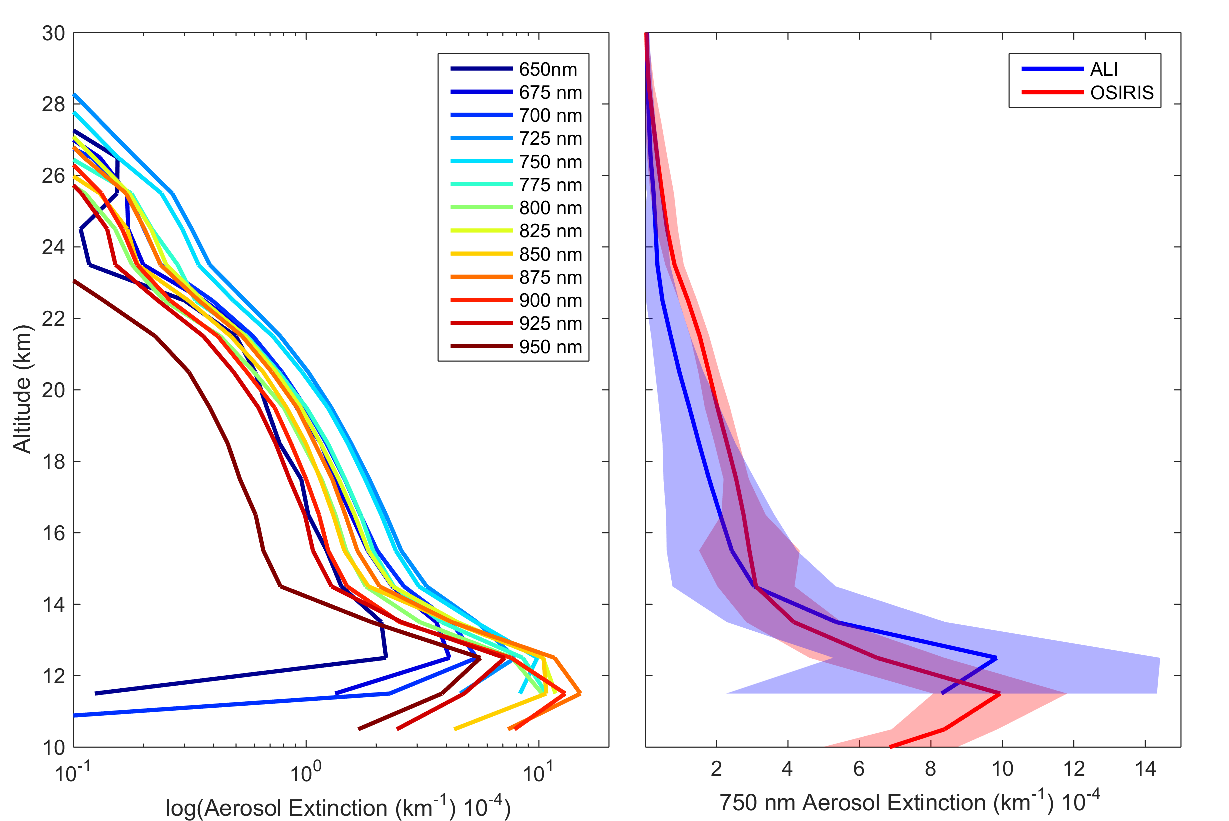
\includegraphics[width=120mm]{amt-2015-329-discussions-f12.pdf}
\caption{Left is the retrieved aerosol extinction profiles from the
  last complete imaging cycle consisting of images 205 to 216 from the
  0.0$^{\circ}$ horizontal line-of-sight. Right is the 750\,nm
  ALI aerosol extinction in blue compared to the 750\,nm extinction measured by OSIRIS
  in red with its error represented by the respective
  shading.}
\label{amtd-2015-0329-f12.pdf}
\end{figure}

\end{document}

